 \section{Fukushima}

In the part, we were given a sample of leaves an gras from the region of Fukushima, which was contaminated with Caesium following the Fukushima nuclear disaster (11.03.2011).
The task was to calculate the date of the disaster, by using the activity ratio of $\frac{^{134}Cs}{^{137}Cs}$ from the sample.
In Fig. \ref{fukushima_spectrum} we can see the measured spectrum of the sample, where we again substracted background radiation.
\begin{figure}[h]
  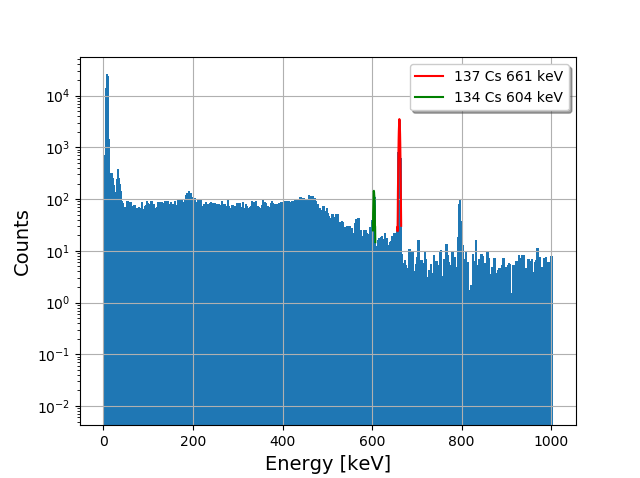
\includegraphics[width=\linewidth]{../Plots/fukushima_spektrum.png}
  \caption{Spectrum of the measured sample.}
  \label{fukushima_spectrum}
\end{figure}
Main interest in this spectrum lies in the peaks from $^{134}$ Cs, with $604$ keV and $^{137}$Cs with $661$ keV, which are marked in Fig. \ref{fukushima_spectrum}.
To calculate the age of the sample, we use the ratio of the activity of $\frac{^{134}Cs}{^{137}Cs}$:
\[
\frac{A_{134}}{A_{137}} = \frac{A_{134}^0}{A_{137}^0} \cdot \frac{e^{-t(\lambda_{134})}}{e^{-t(\lambda_{137})}}
\]
\[
= \frac{A_{134}^0}{A_{137}^0} \cdot e^{-t (\lambda_{134} - \lambda_{137})}
\]
\begin{equation}
\rightarrow t = \frac{ \text{ln} \left(\frac{A_{134} A_{137}^0}{A_{137} A_{134}^0}\right)}{\lambda_{134} - \lambda_{137}}
\label{time}
\end{equation}
With the acitivities of the isotopes during the measurement $A_i$, the acitivities during the accident $A_{i}^0$ and the decay rates $\lambda _i$.
The acivity at any point can be calculated as:
\begin{equation}
A_i (t) = \lambda \cdot N_i (t)
\end{equation}
With the number of particles $N_i$.
Putting this into Eq. \ref{time} gives us:
\begin{equation}
\rightarrow t = \frac{ \text{ln} \left(\frac{A_{134} N_{137}^0 \lambda_{134}}{A_{137} N_{134}^0 \lambda_{137}}\right)}{\lambda_{134} - \lambda_{137}}
\end{equation}
Which means, that we only need to know the abundance ratio of the isotopes.
This can be calculated with the production of these through fission and was given to us as: 
\[
 \frac{^{134}Cs}{^{137}Cs} = \frac{6 \%}{68\%}
\]
The activity of the sample was calculated with:
\begin{equation}
A_i = \frac{N_{obs}}{t_{live} \eta (E_i) P}
\end{equation}
With the area under the Peak $N_{obs}$, calculated with Eq. \ref{gauss_area}, the live time of the detector ($t_{live}=39508 \text{s}$), the peak efficiency for this energy ($\eta$), calculated with Eq. \ref{peak_eff_eq}  and the probabilities of the decays.
For the values in the calculation, we got:
\begin{table}[h]
\centering
\begin{tabular}{c |c | c |c }
\hline
$\text{Isotop}$ & $ \eta $ & $ A[\text{Bq}] $  & $ \lambda $ \\
\hline
$^{137}Cs$ & $(6.79 \pm 0.27) \cdot 10^{-3}$ & $46.353 \pm 0.098$ & $7.302 \cdot 10^{-10}$ \\
$^{134}Cs$ & $(7.64 \pm 0.14) \cdot 10^{-2}$ & $1,29 \pm 0.25$ & $1.064 \cdot 10^{-8}$ \\
\end{tabular}
\caption{Values for the calculation of $t$}
\end{table}
The probabilities were taken from(iaea einfügen) as: $P(604 \text{keV}) = 97 \%$ and $P(661 \text{keV}) = 85 \%$.

Putting this all together gives us:
$t = 11.83 \pm 0.20 \text{a}$
With the day of measurement (14.01.22), this would date the fukushima accident to the 14.03.2010.


